\documentclass[10pt,twocolumn,letterpaper]{article}

\usepackage{tex/cvpr}
\usepackage{times}
\usepackage{epsfig}
\usepackage{graphicx}
\usepackage{amsmath}
\usepackage{amssymb}

% Include other packages here, before hyperref.

% If you comment hyperref and then uncomment it, you should delete
% egpaper.aux before re-running latex.  (Or just hit 'q' on the first latex
% run, let it finish, and you should be clear).
\usepackage[pagebackref=true,breaklinks=true,letterpaper=true,colorlinks,bookmarks=false]{hyperref}

\usepackage{times}
\usepackage{helvet}
\usepackage{courier}
\usepackage{graphicx}
\usepackage{bm}
\usepackage{amsmath,amssymb} % define this before the line numbering.
\usepackage{color}
%\usepackage[width=122mm,left=12mm,paperwidth=146mm,height=193mm,top=12mm,paperheight=217mm]{geometry}
\usepackage{bbm}
\usepackage{epstopdf}
\usepackage{caption}
\usepackage{subcaption}
\usepackage{enumitem}
\usepackage{calc}
\usepackage{multirow}
\usepackage{xspace}
\usepackage{booktabs}
\usepackage{mathrsfs}
\usepackage{array}
\usepackage[font=small,skip=4pt]{caption}

\newcommand{\figref}[1]{Fig\onedot~\ref{#1}}
\newcommand{\equref}[1]{Eq\onedot~\eqref{#1}}
\newcommand{\secref}[1]{Sec\onedot~\ref{#1}}
\newcommand{\tabref}[1]{Tab\onedot~\ref{#1}}
\newcommand{\thmref}[1]{Theorem~\ref{#1}}
\newcommand{\prgref}[1]{Program~\ref{#1}}
\newcommand{\algref}[1]{Alg\onedot~\ref{#1}}
\newcommand{\clmref}[1]{Claim~\ref{#1}}
\newcommand{\lemref}[1]{Lemma~\ref{#1}}
\newcommand{\ptyref}[1]{Property\onedot~\ref{#1}}
\newcommand{\ve}[1]{{\mathbf #1}} % for displaying a vector or matrix
\newcommand{\hua}[1]{{\mathcal #1}}
\newcommand{\scr}[1]{{\mathcal #1}}
\newcommand{\by}[2]{\ensuremath{#1 \! \times \! #2}}
\newcommand{\thickhline}{%
    \noalign {\ifnum 0=`}\fi \hrule height 1pt
    \futurelet \reserved@a \@xhline
}


%\makeatletter
\DeclareRobustCommand\onedot{\futurelet\@let@token\@onedot}
\def\onedot{\ifx\@let@token.\else.\null\fi\xspace}
\def\eg{\emph{e.g.}} 
\def\Eg{\emph{E.g}\onedot}
\def\any{\forall}
\def\ie{\emph{i.e.}} 
\def\Ie{\emph{I.e}\onedot}
\def\cf{\emph{cf}\onedot} 
\def\Cf{\emph{Cf}\onedot}
\def\etc{\emph{etc}\onedot} 
\def\vs{\emph{vs}\onedot}
\def\wrt{w.r.t\onedot} 
\def\dof{d.o.f\onedot}
\def\etal{\emph{et al.}}

\cvprfinalcopy % *** Uncomment this line for the final submission
\pagenumbering{gobble}
\def\cvprPaperID{****} % *** Enter the CVPR Paper ID here
\def\httilde{\mbox{\tt\raisebox{-.5ex}{\symbol{126}}}}

% Pages are numbered in submission mode, and unnumbered in camera-ready
\ifcvprfinal\pagestyle{empty}\fi
\begin{document}
%%%%%%%%% TITLE
\title{Activity driven objection detection by learning from videos}

\author{
Zhenheng Yang$^{1}$~~Vignesh Ramanathan$^{2}$~~Deepti Ghadiyaram$^{2}$~~Dhruv Mahajan$^{2}$~~Ram Nevatia$^{1}$\\
\\
% \texttt{
% zhenheny@usc.edu~\{wangpeng54,wangyang59,wei.xu\}@baidu.com~nevatia@usc.edu}\\
$^{1}$University of Southern California~~$^{2}$Facebook Research~~\\
}

\maketitle
%\thispagestyle{empty}


\begin{abstract}
    Weakly supervised object detection is attracting significant attention as it does not require tedious bounding box annotation. There have been exsiting works which focus on learning object appearance representation from static images. However, they often fail to generalize to objects in videos because of domain shift. In this work, we investigate the problem of weakly supervised object detection with the supervision from video-level interactive activity class annotations. 

    Different from learning solely from static images, appereance consistency over time can be leveraged in videos. More importantly, the object apperance representation is further regularized by jointly modeling the appereance information with different activity classes which involve the same object category. 
    We have conducted comprehensive experiments on Charades and (potentially MPII-Cooking) dataset and achieve () performance. To validate the performance of generalization, (the proposed method) is directly tested on (Pascal VOC) dataset and shows superior performance over other baselines.
\end{abstract}

% % \vspace{-0.6\baselineskip}
\section{Introduction}
% \vspace{-0.4\baselineskip}
\label{sec:intro}

With the advances of deep learning techniques and increase in dataset collections, there have been successes in scaling up object classification systems. However, unlike object class labeling, tedious bounding boxes annotation, which is required for supervised object detection, is hardly scalable. 
% Besides, videos provide richer information than static images and can be leveraged for learning. 
Recently, there have been impressive progresses in unsupervised and weakly supervised object detection, making the pipeline free of bounding box supervision. However, existing unsupervised methods show much inferior performance compared to supervised methods. And the weakly supervised ones, which are mostly trained on static images, often fail to generalize to videos due to domain shift. In light of this, we investigate the problem of ``weakly supervised object detection by learning from videos with action labels''. Instead of using boudning box annotations in fully-supervised pipeline or video-level object class in previous weakly supervised method, we use video-level action class annotation for supervision, as it is easy to obtain and commonly appears in existing video datasets. During training, only videos with action labels are used. For evaluation, static images are fed into the pipeline and spatial bounding boxes with object classes will be estimated.

% \begin{figure}
% % \vspace{-0.5\baselineskip}
% 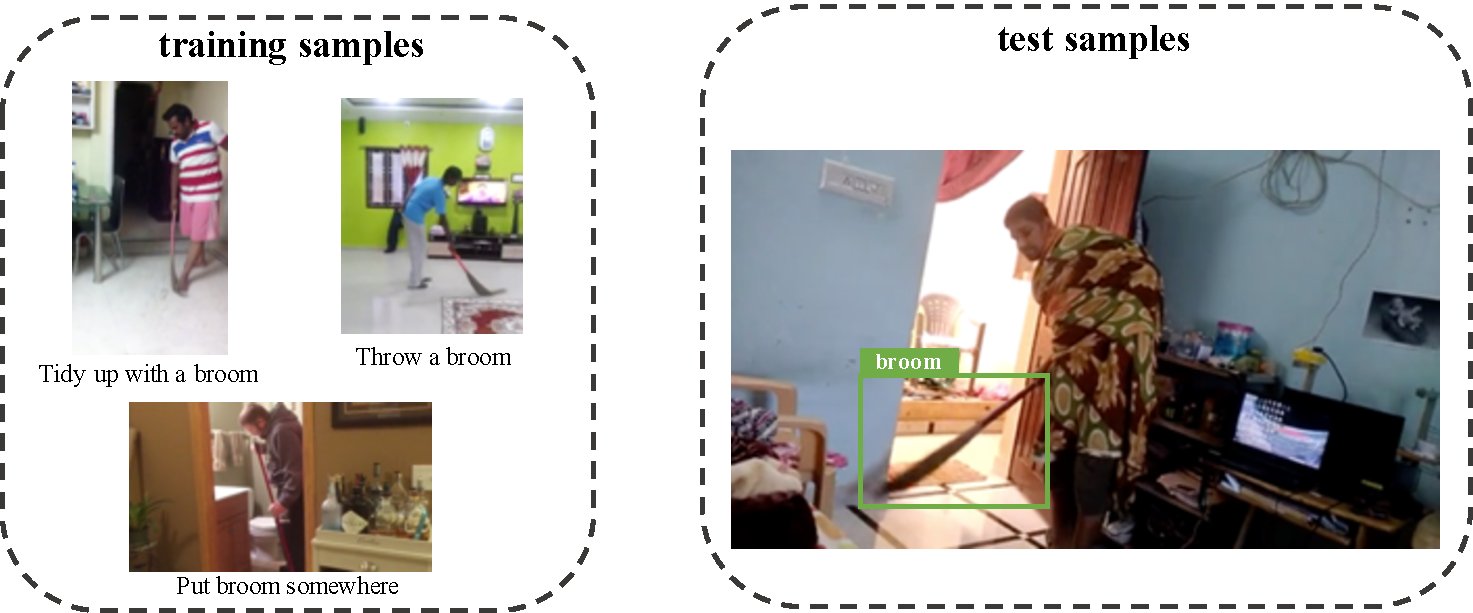
\includegraphics[width=0.5\textwidth]{figures/training_test_samples.pdf}
% % \caption{Visual comparison of depth and normal results between \protect\cite{zhou2017unsupervised} and ours. As the original depth ground truth map comes from sparse laser measurement, the interpolated depth map is shown for better visualization. As can be seen from the depth estimation, our results preserve the small/thin structures which have similar color to other foregrounds (green circles). From the normal comparison, our results predict the road normal direction better and have no artifact. The edges in normal map are also preserved better in our results (yello circles).}
% \caption{Train samples include videos with action labels. Bounding boxes and object class are estimated during evaluation.}
% % \vspace{-0.8\baselineskip}
% \label{fig:train_samples}
% \end{figure}

\begin{figure*}
% \vspace{-0.5\baselineskip}
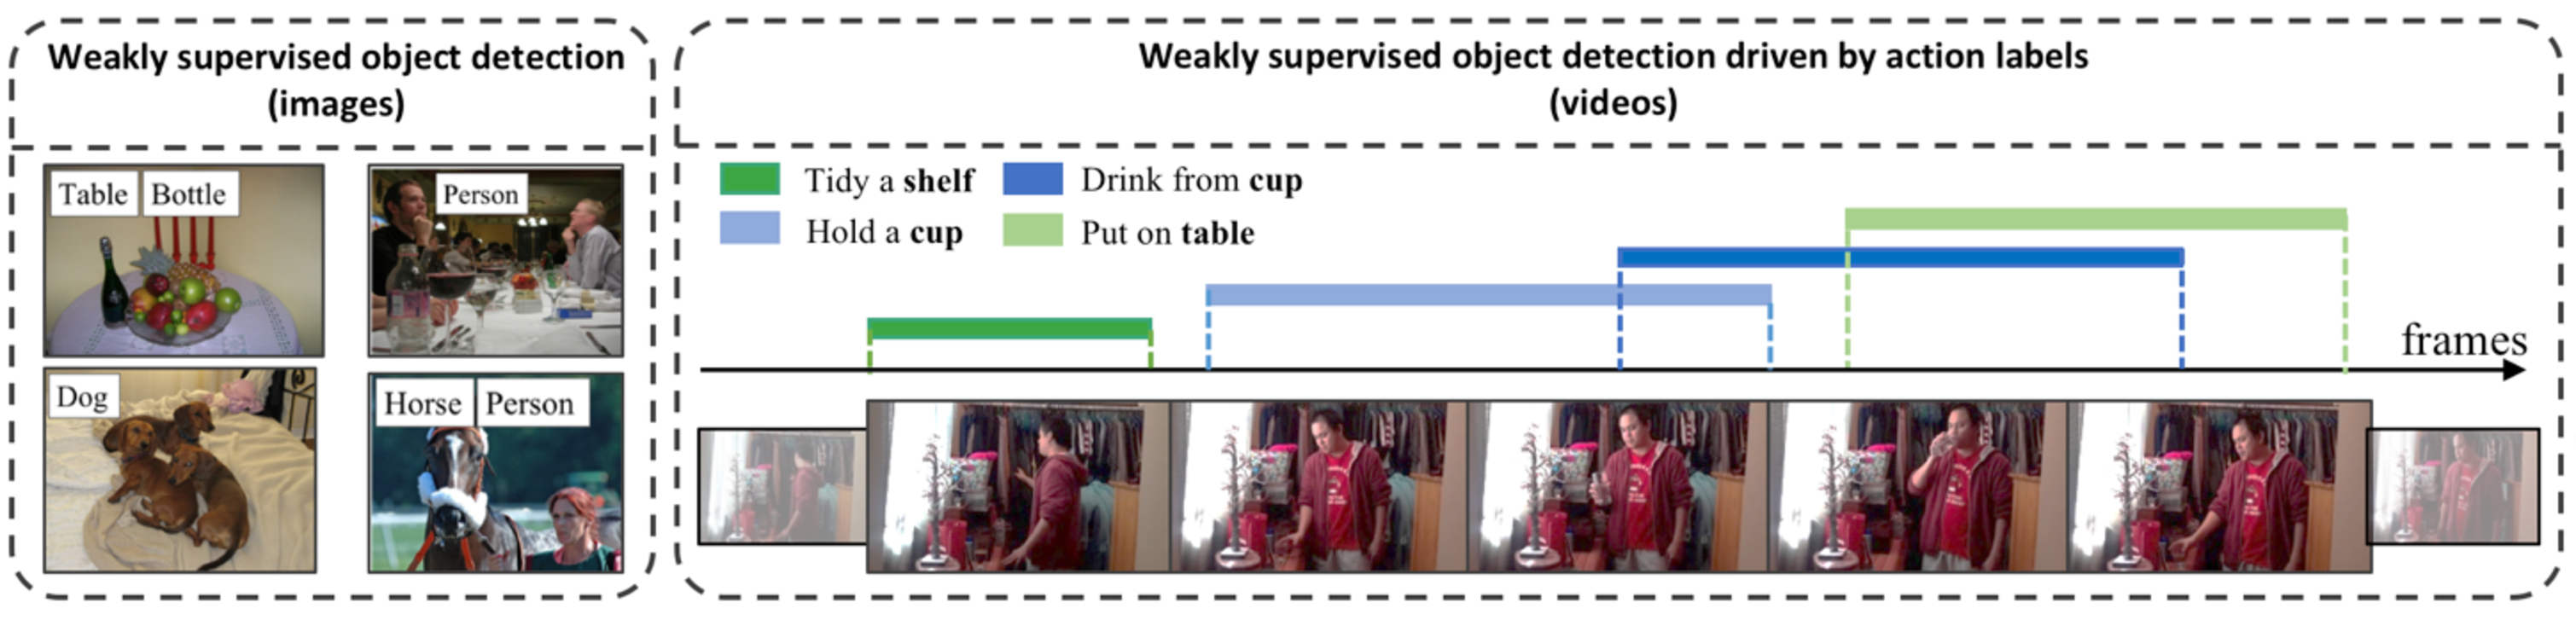
\includegraphics[width=1.0\textwidth]{figures/task_definition.pdf}
% \caption{Visual comparison of depth and normal results between \protect\cite{zhou2017unsupervised} and ours. As the original depth ground truth map comes from sparse laser measurement, the interpolated depth map is shown for better visualization. As can be seen from the depth estimation, our results preserve the small/thin structures which have similar color to other foregrounds (green circles). From the normal comparison, our results predict the road normal direction better and have no artifact. The edges in normal map are also preserved better in our results (yello circles).}
\caption{Traditional weakly supervised object detection takes images with image-level object classes as training samples. Our task takes video with clip-level action labels as ground truth for training.}
% \vspace{-0.8\baselineskip}
\label{fig:task_definition}
\end{figure*}

Previous work \cite{yuan2017temporal} proposed to cope with the problem by leveraging temporal consistency of object proposals and use the object class that appears in the action name (\eg ``cup'' in the action ``drink from cup'') as video-level object labels for supervising the learning of object appearance. Specifically, the class-agnostic object proposals are generated using EdgeBoxes \cite{zitnick2014edge}. The proposals are linked in temporal space by measuring the appearance feature similarity. The appearance feature is updated recurrently by incorporating the information from neighboring frames using LSTM. The updated features are then fed into a two-stream classification module as in \cite{bilen2016weakly} and the related object class in action label is used for classification supervision. Such method only parses the object class from action class labels and fails to model the human action motion or the interaction between human and objects.

In this work, we are solving the drawbacks mentioned above. Our ideas are mainly motivated by three observations: (1) The object appearance is consistent across videos and across action classes which involve the same object class; (2) There is spatial correlation between the motions of objects and human key points, \eg in action ``hold cup'', the location of cup is tightly correlated with location of the hand. And such correlation is dependent on action class; (3) The most informative object in the scene of a certain action class is the interacted object and thus the action class can be leveraged for object appearance modeling. The most dominant challenge in this task is the large space and few supervision signal. We try to formulate our proposed method to decrease the search space based on the above observations: (1) use generic object classifier for modeling object appearances, (2) learn an attention ditribution to model the probability of object locations \wrt the human joint, (3) jointly learn action and object classification to leverage the action cues.

We conducted comprehensive experiments over the Charades dataset \cite{sigurdsson2016hollywood} and show that our method outperforms the previous methods \cite{bilen2016weakly,yuan2017temporal} by a large margin on both detection and classification tasks. On object detection task, we have achieved an absolute 4\% boost in mAP, from current SOTA 1.98\% to 5.94\%. Ablation experiments show the effectiveness of each module in our proposed approach and robustness to the selection of hyper-parameters.

% 
\vspace{-0.5\baselineskip}
\section{Related Work}
\vspace{-0.5\baselineskip}
\label{sec:related}
%\vspace{-0\baselineskip}
In this section, we briefly overview some traditional methods, and introduce current SOTA methods for unsupervised single view 3D geometry recovery and edge detection. 

\textbf{~Structure from motion and single view geometry.}
Geometric based methods estimate 3D from a given video with feature matching, such as SFM~\cite{wu2011visualsfm}, SLAM~\cite{mur2015orb,engel2014lsd} and DTAM~\cite{NewcombeLD11}, which could be effective and efficient in many cases. 
However, they can fail at where there is low texture, or drastic change of visual perspective \etc. More importantly, it can not extend to single view reconstruction.
Specific rules are developed for single view geometry, such as computing vanishing point~\cite{HoiemEH07}, following rules of BRDF~\cite{prados2006shape,kong2015intrinsic}, or extract the scene layout with major plane and box representations~\cite{DBLP:conf/iccv/SchwingFPU13,DBLP:conf/3dim/SrajerSPP14} \etc. These methods can only obtain sparse geometry representations, and some of them require certain assumptions (\textit{e.g.} Lambertian, Manhattan world).

\textbf{Supervised single view geometry via CNN.}
Deep neural networks (DCN) developed in recent years, \eg VGG~\cite{simonyan2014very} and ResNet~\cite{laina2016deeper}, provide strong feature representation. Dense geometry, i.e., pixel-wise depth and normal maps, can be readily estimated from a single image~\cite{wang2015designing,eigen2015predicting,laina2016deeper,li2017two,chuang2018cvpr}. The learned CNN model shows significant improvement compared to other methods based on hand-crafted features~\cite{karsch2014depth,ladicky2014pulling,zeisl2014discriminatively}. Others tried to improve the estimation further by appending a conditional random field (CRF)~\cite{DBLP:conf/cvpr/WangSLCPY15,Liu_2015_CVPR,li2015depth}. Recently, Wang \etal \cite{peng2016depth} proposed a depth-normal regularization over large planar surfaces, which is formulated based on a dense CRF~\cite{DBLP:journals/corr/abs-1210-5644}, yielding better results on both depth and normal predictions. However, all these methods require densely labeled ground truths, which are expensive to obtain in natural environments.

 % Long-range context and semantic cues are also incorporated in later works to refine the dense prediction by combining the networks with conditional random fields (CRF)~\cite{DBLP:conf/cvpr/WangSLCPY15, Liu_2015_CVPR, li2015depth, Wang_2015_CVPR}. Most recently, Eigen \textit{et al.}~\cite{DBLP:conf/iccv/EigenF15} further integrate depth and normal estimation into a large multi-scale network structure, which significantly improves the geometry estimation accuracy. Nevertheless, the output of the networks still lacks regularization over planar surfaces due to the adoption of pixel-wise loss functions during network training, resulting in unsatisfactory experience in 3D image editing applications.


%Later, the depth estimation from single-view input image is inherently an ill-posed problem which can only be solved with priors and semantic understanding of the scene - tasks that the convnets are good at. 
% There is a chain of works that propose learning depth/normal maps with deep convnets supervised with dense ground truth maps. \cite{liu2016learning} proposed to combine a convnet with a superpixel-based conditional random field (CRF) model, and to learn unary and pairwise terms for the depth map. Ladicky \etal \cite{ladicky2014pulling} incorporate semantics into their model to improve the per pixel depth estimation. Karsch \etal \cite{karsch2014depth} attempt to produce more consistent image level predictions by copying whole image depth from the training set, which requires the entire training set to be available during test time. Eigen \etal \cite{eigen2014depth,eigen2015predicting} showed it is possible to produce dense per pixel depth estimation through a two-scale deep network, trained on images and their corresponding ground truth depth maps. Many works have built upon this method using techniques like CRFs to improve accuracy \cite{li2015depth}, replacing regression loss with classification loss \cite{cao2017estimating}, implementing more robust loss function \cite{laina2016deeper}.

% Wang \etal \cite{wang2015designing} also built upon the basic idea of \cite{eigen2014depth} and incorporate scene geometrical priors to help learning, in the related problem of normal estimation. Data-driven normal estimation has not been long since the first approach, that directly tries to estimate surface normals from the data was proposed by Fouhey \etal \cite{fouhey2013data}.  Both this work and \cite{zeisl2014discriminatively} proposed by Ladicky \etal used hand-crafted features like texton, SIFT, local quantized ternary patterns. Li \etal \cite{\cite{li2015depth}} first proposed to estimate depth and normal jointly and showed performance gain. 

\textbf{Unsupervised single view geometry.}
Motivated by traditional methods, videos, which are easier to obtain and hold richer 3D information. Motivated by traditional methods like SFM and DTAM, lots of CNN based methods are proposed to do single view geometry estimation with supervision from vieos, and yield impressive progress. 
 Deep3D \cite{xie2016deep3d} learns to generate the right view from the given left view by supervision of stereo image pairs. In order to do back-propagation on depth values, the depth space is quantized and it is trained to select the right depth value. 
% Video holds a great potential towards semantically meaningful visual representations. Recently, there have been a small number of deep network based methods for depth estimation. 
% DeepStereo \cite{flynn2016deepstereo} introduced a novel view synthesis network, while . This network generates new view images by selecting pixels from nearby images. The most appropriate depth values are selected to sample pixel values from neighboring images, based on plane sweep volume.
Concurrently, Garg \etal \cite{GargBR16} applied the similar supervision from stereo pairs, while the depth is kept continuous. They apply Taylor expansion to approximate the gradient for depth. Godard \etal \cite{godard2016unsupervised} extend Garg's work by including depth smoothness loss and left-right depth consistency. 
Zhou \etal \cite{zhou2017unsupervised} incoporated camera pose estimation into the training pipeline, which made depth learning possible from monocular videos. And they came up with an explainability mask to relieve the problem of moving object in rigid scenes.
%However, they only focus on rigid scene without the ability to deal with moving objects. 
At the same time, Vijayanarasimhan \etal \cite{Vijayanarasimhan17} proposed a network to include the modeling of rigid object motion. Most recently, Yang \etal \cite{yang2018aaai} further induce normal representation, and proposed a dense depth-normal consistency within the pipeline, which not only better regularizes the predicted depths, but also learns to produce a normal estimation. However, as discussed in \secref{sec:intro}, the regularization is only applied locally and can be blocked by image gradient, yielding false geometrical discontinuities inside a smooth surface.

% bilateral filter, dense crf
\textbf{Non-local smoothness.} Long range and non-local spatial regularization has been vastly explored in classical graphical models like CRF~\cite{lafferty2001conditional}, where nodes beyond the neighboring are connected, and the smoothness in-between are learned with high-order CRF~\cite{ye2009conditional} or densely-connected CRF~\cite{DBLP:conf/icml/KraehenbuehlK13}. They show superior performance in detail recovery than those with local connections in multiple tasks, \eg segmentation~\cite{DBLP:journals/corr/abs-1210-5644}, image disparity~\cite{scharstein2007learning} and image matting~\cite{chen2013image} \etc In addition, efficient solvers are also developed such as fast bilateral filter~\cite{barron2016fast} or permutohedral lattice~\cite{adams2010fast}. 

Although these methods run effectively and could combine with CNN as a post processing component~\cite{arnab2016higher,crfasrnn_iccv2015,peng2016depth,wang2017occlusion}, they are not very efficient in learning and inference when combined with CNN, due to the iterative loop. To some extent, the non-local information from CRF overlaps with those multi-scale strategies~\cite{zhao2016pyramid,ChenPSA17} proposed recently, which yield comparable performance while are more effective. Thus, we adopt the latter strategy to learn the non-local smoothness inside the unsupervised pipeline, which is represented by geometrical edge in our case.


\textbf{Edge detection.}
Learning edges from an image beyond low level methods such as Sobel or Canny~\cite{canny1986computational} has long been explored via supervised learning~\cite{yamaguchi2012continuous,konishi2003statistical,arbelaez2011contour,DollarICCV13edges} along with the growth of semantic edge datasets~\cite{MartinFTM01,hou2013boundary}. Recently, methods~\cite{bertasius2015high,xie2015holistically,DBLP:journals/corr/Kokkinos15} have achieved outstanding performance by adopting supervisedly trained deep features. 

As discussed, high-level edges can also be learned through non-local smoothness by implicit supervision. One recent work close to ours is \cite{chen2016semantic}. They append a spatial domain transfer (DT) component after a CNN, which acts similar to a CRF for smoothness, and improves the results of semantic segmentation. However, their work is fully supervised with ground truth, and similar to CRF, the DT propagates to neighboring pixels every iteration which is not efficient. When no supervision is provided, Li \etal \cite{li2016unsupervised} proposed to use optical flow~\cite{revaud2015epicflow} to explicitly capture motion edge and use it as supervision for edge models. 

Our method discovers geometrical edges in an unsupervised manner. In addition, we show that it is possible for the network to directly extract edge and smoothen the 3D geometry by enforcing a unified regularization, without appending extra components like~\cite{chen2016semantic}. We also show better performance than~\cite{li2016unsupervised} in street-view cases. 
% Lastly, joint with 3D geometry, our edges also contain the information of occlusion which is also full of interest in computer vision~\cite{HoiemEH11,DBLP:conf/cvpr/SundbergBMAM11,wang2016doc}.
% also learning with video

%The edge detection task has a long history. Early edge detection methods were manually designed to use simple convolutional filters such as Sobel \cite{} or Canny \cite{}. More recent works have proposed edge detectiors trained with a data driven manner. Dollar \etal \cite{DollarICCV13edges} proposed a realtime edge detection method using trained structured random forests (SE). With the advances of deep neural network, the performance of dense edge prediction is boosted. A notable work by Xie \etal \cite{xie2015holistically} proposed a holistically-nested edge detector (HED) which trains and predicts the edge in an image-to-image fashion and performs end-to-end-training.  
% To avoid tedious edge ground truth labeling, Li \etal \cite{Li2016unsupervised} proposed to learn motion edge from videos and use the optical flow edges as intermediate ground truth to supervise the training of SE.

% Although there have been many efforts devoted to unsupervised learning of 3D geometry, the geometry consistency, like depth and normal consistency, geometric edge and depth/normal consistency have not been explored in the pipeline. Our work fills in this part and show that edges serve as an important intermediate regularization for 3D geometry learning. 
% Although vastly developed for depth estimation from video, normal information, which is also highly interesting for geometry prediction, has not been considered inside the pipeline. This paper fills in the missing part, and show that normal can serve as a natural regularization for depth estimation, which significantly improves the state-of-the-art performance. Finally, with our designed loss, we are able to learn the indoor geometry where \cite{zhou2017unsupervised} usually fails to estimate.

% To deal with the problem of occlusion boundary caused by the rigid scene transformation and moving object, they proposed to mask out all these boundaries.

% \input{preliminaries}
% % \input{approach_new}
% % \vspace{-0.4\baselineskip}
\section{Approach}
% \vspace{-0.4\baselineskip}
\label{sec:approach}

\begin{figure*}[ht!]
\centering
% \vspace{-0.5\baselineskip}
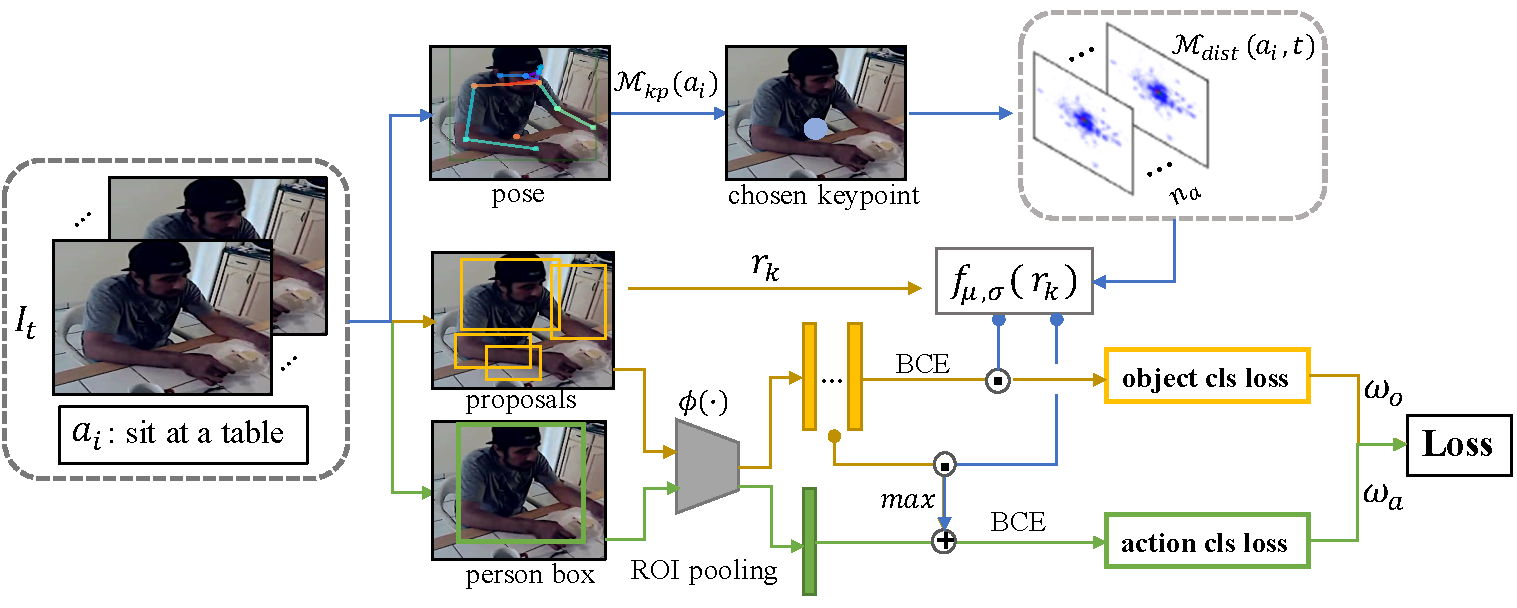
\includegraphics[width=0.8\textwidth]{figures/pipeline.pdf}
% \caption{Visual comparison of depth and normal results between \protect\cite{zhou2017unsupervised} and ours. As the original depth ground truth map comes from sparse laser measurement, the interpolated depth map is shown for better visualization. As can be seen from the depth estimation, our results preserve the small/thin structures which have similar color to other foregrounds (green circles). From the normal comparison, our results predict the road normal direction better and have no artifact. The edges in normal map are also preserved better in our results (yello circles).}
\caption{The object appearance is learned with a weakly supervised method by leveraging the three regularizations.}
% \vspace{-0.8\baselineskip}
\label{fig:pipeline}
\end{figure*}
% As discussed in \secref{sec:intro}, one major problem is that both~\cite{zhou2017unsupervised} and~\cite{yang2018aaai} have the regularization performed \wrt image gradient, which blocks nonlocal smoothness due to many false positives such as boundaries of shadows. 
In this section, we introduce the framework and different regularizations we have applied in detail.
\subsection{Overview}
% In this section, we introduce the regularizaitons we apply to learn the object representation via supervision from action labels. To better show our analysis, the information that can be leveraged are listed in different axis in \figref{fig:analysis}. Basically, we propose to explore three constraints to help learning object appearance. The first one includes the appearance consistency of objects in the same action class (blue box in \figref{fig:analysis}). The other constrain comes from the motion consistency in the same action class. The motion of ``drinking water from cup/bottle'', including both subject and object motion, is similar across videos. Last but not least, the object appears similarly in videos of different action labels but involving same object category. In the actions ``holding vacuum'' and ``fixing vacuumm'' (green box in \figref{fig:analysis}), object appearances are consistent.
As stated before, we propose to leverage appearance and motion consistency in the interaction between person and objects. The motion consistency is modeled by modeling the correlation between spatial location change with time, between person and interacted objects. Practically, such correlation is modeled between the person joint and object locations. The person joints (keypoints) are firstly estimated with off-the-shelf method and a dominant keypoint is chosen automatically by the pipeline. Attention maps around the chosen keypoint are estimated to model the probability of object locations. Class agnostic proposals are generated in a bottom-up way and weighted with the attention maps. The weighted proposals are then fed into action classification and object classification modules respectively. The action classification module takes object proposals and person detection bounding box as input and outputs action classification scores. Binary cross-entropy loss is calculated as supervision. Object classification module takes proposals as input and logistic losses are calculated for each object class as supervision. The weighted sum of the two losses is the final loss for the whole framework. 

\subsection{Framework}

Formally, for a given training video, the provided annotations include a set of action labels $\scr{L}$ = {$l_1,...,l_n$}. Each action label consists of an action class $a_i$ and corresponds to a clip in the video. The action class $a_i$ belongs to a predefined action set $a_i \in \scr{A}$, which is of size $n_{a}$: $||\scr{A}||=n_{a}$. All actions are interactive and there is one object class involved in the action $a_i\rightarrow o_{m(i)}, o_{m(i)}\in \scr{O}$. For example, object class \textit{cup} appears in the action \textit{holding a cup}. $m$ is a mapping from action class to object class. There are $n_{o}$ object classes: $||\scr{O}||=n_{o}$ in total. During training, clip-level action class $a_i$ and corresponding object class $o_j$ are used as supervision signal.

\figref{fig:pipeline} illustrates an overview of our approach. $\scr{F}$ frames are uniformly sampled from each clip and are processed with a person detector and pose estimation network to generate person bounding box $P_t$ and human key point detection results $K_t$ for each frame $f_t$. Class-agnostic proposals $R_t$ are also generated as candidate bounding boxes. To model the correlation between action and object motion, a keypoint is automatically chosen for a given action class. A spatial distribution is estimated to model the probability of object's spatial location with time. All proposals $R_t$ and person bounding box $P_t$ are processed with a convolutional network to extract appearance features. Proposal features are firstly fed into the object classification module and $n_o$-dimension classification scores are generated for each proposal region. The cross-entropy classification losses are weighted with the probability mentioned above and used as supervision from object classification. 

The action class labels are leveraged in the action classification stream. The person bounding box is processed with the same convolutional network to extract the person visual features $\phi(P_t)$. Similar to the multiple instance learning idea in \cite{gkioxari2015contextual}, the person region feaures are fused with the proposal region features $\phi(R_t)$ and then fed into the action classification module. As shown in \figref{fig:task_definition}, there may be overlap between different annotated clips, and thus it poses the action classification as a multi-label problem. The binary cross-entropy loss is used as action classification supervision. The object and action classification losses are weighted summed as the final loss term.

\subsection{Object classification}
The features are extracted for each proposal region $\phi(r_k), r_k \in R_t$ (superscript $t$ is omitted in $r_k^t$ for simpler symbol) and there are $K$ proposals on frame $f_t$: $||R_t||=K$. An $n_o$-dimensional classification score is generated by applying object classification fully connected (\textit{fc}) layer on appearance features: $S_o(r_k) = fc_o(\phi(r_k))$ for each proposal. As mentioned in the last section, there can be multiple action and object classes labels for one frame. Assume for frame $f_t$, there is a set of action labels $\scr{A}_t$ and object labels $\scr{O}_t$. Given action class $a_{i_t} \in \scr{A_t}$ and time stamp $t$, a key point is selected based on the action class $\hua{I} = \hua{M}_{kp}(a_{i_t})$ and a distribution is estimated $(\mu_{i_t}, \sigma_{i_t}) = \hua{M}_{dist}(a_{i_t}, t)$ with regard to $\scr{K}_t(\hua{I})$. $\mu_{i_t}, \sigma_{i_t} \in \scr{SE}^2$, indicating the mean and variance in 2D space respectively. Based on the estimated probability distribution $\scr{N}_{(\mu_{i_t}, \sigma_{i_t})}$ for given action class of one frame, each proposal is assigned with a probability $N_{(\mu_{i_t}, \sigma_{i_t})}(r_k), k\in [1,...,K]$. The object classification loss on frame $f_t$ is formally:
\begin{align}
\label{eqn:obj_cls_loss}
&\hua{L}_{obj} (f_t) = -\frac{1}{K\cdot |\scr{A}_t|}\sum_{a_{i_t}\in {A_t}}\sum_{k=1}^{K} N_{(\mu_{i_t}, \sigma_{i_t})}(r_k) \cdot \nonumber \\
&~~~~~~~~~~~~~~~~~~~~~~~~~~~~~~~log(P(\alpha=o_{m(i_t)}|r_k, f_t)), \nonumber\\
&P(\alpha|r_k, f_t) = \frac{exp(S_o(r_k)_{\alpha}}{\sum_{\alpha \in \scr{O}}exp(S_o(r_k)_\alpha)}, \alpha \in \scr{O}
\end{align}

\subsection{Action classification}
For the task of action recognition, especially for interactive actions as in our task, both the person and the object appearances are vital cues. As indicated in \cite{gkioxari2015contextual}, the spatial location of the most informative object, which is often the one that the person interacted with, can be mined from action recognition task. We incorporate similar idea into our pipeline by introducing a separate action classification stream to help learn the object appearance. Formally, on given frame $f_t$ in a clip, the appearance features of both person region $p$ and proposal regions $r$ are extracted and then linearly transformed into an $n_a$-dimensional score: $S_a^o(r_k) = fc_a^o(\phi(r_k))$ and $S_a^a(P_t) = fc_a^a(\phi(P_t))$. For each action class $a_{i_t} \in \scr{A}_t$, the weighted sum of proposal classification scores is added with person region classification score as a combined score. And the cross-entropy loss for each action class is averaged as the action classification loss. The formulation is shown in \equref{eqn:act_cls_loss}.

\begin{align}
\label{eqn:act_cls_loss}
&\hua{L}_{act} (f_t) = -\frac{1}{\scr{K}\cdot |\scr{A}_t|}\sum_{a_{i_t}\in {A_t}}\sum_{k=1}^{K} N_{(\mu_{i_t}, \sigma_{i_t})}(P_k) \cdot \nonumber \\
&~~~~~~~~~~~~~~~~~~~~~~~~~~~~~~~log(P(\alpha=a_{i_t}|r_k, f_t)), \nonumber\\
&P(\alpha|r_k, f_t) = \frac{exp(S_a^a(r_k)_{\alpha}+S_a^o(r_k)_{\alpha}*N_{(\mu_{i_t},\sigma_{i_t})}(r_k))}{\sum_{\alpha \in \scr{A}}exp(S_a^a(r_k)_{\alpha}+S_a^o(r_k)_{\alpha}*N_{(\mu_{i_t},\sigma_{i_t})}(r_k))}
\end{align}

\subsection{Loss terms}
The final loss is a weighted sum of the above loss terms. The hyperparameters $w_o$ and $w_a$ are weights to trade off the relative importance of object classification and action classification in the pipeline.
\begin{align}
\label{eqn:final_loss_term}
\hua{L}(\scr{F}, \scr{A}, \scr{O}) = \frac{1}{||\scr{F}||}(w_o\hua{L}_{obj}+w_a\hua{L}_{act})
\end{align}


% % \vspace{-0.2\baselineskip}
\section{Evaluation}
% \vspace{-0.3\baselineskip}
\label{sec:evaluation}

We conducted experiments on Charades dataset \cite{sigurdsson2016hollywood}. Charades dataset includes 9848 videos of 157 action classes, among which, 124 actions include interaction with objects. In our experiments, the pipeline is trained on 7342 training videos with action class labes and evaluated on 5,000 test frames with object bounding box annotations \cite{}. The 5,000 frames are randomly picked from 200 test videos. 

Our method is compared with several baseline methods on the same dataset for both the detection (det) and classification (cls) tasks. The baselines include \cite{bilen2016weakly,kantorov2016contextlocnet} which are weakly supervised object detectors learning from static images, \cite{yuan2017temporal} which learns object detector from videos but only leverages the temporal consistency within the same action class, R*CNN \cite{gkioxari2015contextual} with both pretrained model and model trained on Charades data and Faster R-CNN (pretrained and trained on Charades), which is a fully supervised baseline. The performances are presented in Tab. \ref{tbl:sota}. We also compare current SOTA methods on each object class, which is shown in Tab. \ref{tbl:class_wise}.

\begin{table}[]
\fontsize{7}{8}\selectfont
% \def\arraystretch{1.5}
\setlength{\tabcolsep}{3pt}
\centering
\caption{Performances of different baseline methods on object classification and object detection tasks}
\label{tbl:sota}
\begin{tabular}{l|c|cc}
\specialrule{.2em}{.1em}{.1em}
Methods                          & Supervision                          & mAP (det) & mAP (cls) \\ \hline
WSDNN \cite{bilen2016weakly}                            & \multirow{5}{*}{Weak (action class)} & 0.65            & 15.67                \\
ContextLocNet \cite{kantorov2016contextlocnet}                    &                                      & 1.12            & 16.47                \\
TD-LSTM \cite{yuan2017temporal}                          &                                      & 1.98            & 19.52                \\
R*CNN \cite{gkioxari2015contextual} (pre-trained)            &                                      & $0.47\pm 0.02$\footnotemark[1]            &                      \\
R*CNN \cite{gkioxari2015contextual} (re-trained)                 &                                      & $1.26\pm 0.11$             &                      \\ \hline
Faster R-CNN \cite{ren2015faster} (pre-trained)             & \multirow{2}{*}{Strong (bbox)}       & $4.39\pm 0.34$\footnotemark[1]            & -                    \\
Faster R-CNN \cite{ren2015faster} (fine-tuned) &                                      & $63.98\pm 1.13$                & -                    \\ \hline
\end{tabular}
\end{table}
\addtocounter{footnote}{1}
\footnotetext{The test set is slightly different but there should not be large offset in numbers.}

\begin{table}[]
\centering
\caption{Class-wise mAP performance for different methods.}
\label{tbl:class_wise}
\begin{tabular}{l|ccc}
\specialrule{.2em}{.1em}{.1em}
Methods                                        & cup/bottle    & table         & door          \\ \hline
WSDDN \cite{bilen2016weakly}                   & 0.03          & 1.74          & 0.31          \\
ContextLocNet \cite{kantorov2016contextlocnet} & 0.02          & 0.63          & 0.17          \\
TD-LSTM \cite{yuan2017temporal}                & \textbf{0.49} & 3.35          & 1.17          \\ \hline
Ours                                           & 0.28          & \textbf{4.39} & \textbf{2.35} \\ \hline
\end{tabular}
\end{table}

\newpage
% \section{Conclusion}
In this paper, we propose a human pose guided pipeline for activity driven weakly supervised object detection.
Weakly supervised object detection is attracting significant attention as it gets rid of supervision from bounding box annotations, which are expensive and tedious. Exsiting works either focus on learning object appearance representation from static images, which fail to generalize to objects in videos because of domain shift, or only leverage the object class annotations but ignore the action information. In this work, we investigate the problem of weakly supervised object detection with the supervision from video-level action class annotations. We propose to leverage both the object and action class labels during training. Specifically, we leverage the object appearance consistency by applying object classification across different videos or actions which involve the same object class. The temporal consistency is modeled with attention maps which are dependent only on the action class. We also model the action apperance cues by supervision from action class labels. Combining the regularizations above, our method has shown better performance than state-of-the-art (SOTA) methods. We conducted experiments on Charades dataset to compare with baseline methods using the metric of mean Average Precision (mAP) and showed our pipeline outperforms the current SOTA by \%. (To evaluate the generalization capability of our pipeline, we also directly evaluate the model, which is trained on Charades, on different datasets.)

{\small
\bibliographystyle{tex/ieee}
\bibliography{tex/reference}
}

\end{document}
